\section{Data Previews and Data Release 1} 
\label{sec:datapreview}

A series of three Data Previews (DP) are planned  based on commissioning data to support the community as they develop their LSST analysis software and worfklows, and to enable high-impact science as soon as possible.
\begin{itemize}
\item Data Preview 0 (DP0): Based on simulated LSST-like data.
\item Data Preview 1 (DP1): Based on a few nights of early science-grade commissioning data taken with LSSTCam.
\item Data Preview 2 (DP2): Based on a full reprocessing of all science-grade LSSTCam data taken during commissioning.
\end{itemize}

Due to the relatively short time periods available for commissioning observations (\S~\ref{ssec:scenarios}), these Data Previews will necessarily be limited in their area and temporal coverage relative to full a Data Release, however all Data Preview data products will be in the same science data model format as for future Data Releases.

The data products that comprise a Data Preview are produced by the LSST Science Pipelines \citep{2019ASPC..523..521B,2018PASJ...70S...5B}.
For an introduction to the LSST data products, see \citet{RubinDataProductsAbridged} and for a detailed description, see the LSST \dpdd{},  \citedsp{LSE-163}.
Each pre-operations Data Preview and survey Data Release will be accompanied by its own release-specific DPDD\footnote{For an example data release DPDD, see the online DP0.2 documentation {\url{https://dp0-2.lsst.io/data-products-dp0-2/}}.}, giving e.g. the  database schema for the catalogs included in that dataset.

Table~\ref{tab:data-preview-summary} provides a summary of the expected early science data products available in DP0, DP1, DP2 and the LSST Data Release 1, as of January 2023.
In the case of DP1, these expectations come with considerable uncertainty, see Table~\ref{tab:dp-one-products} for more details.

\begin{table}[ht]
\centering
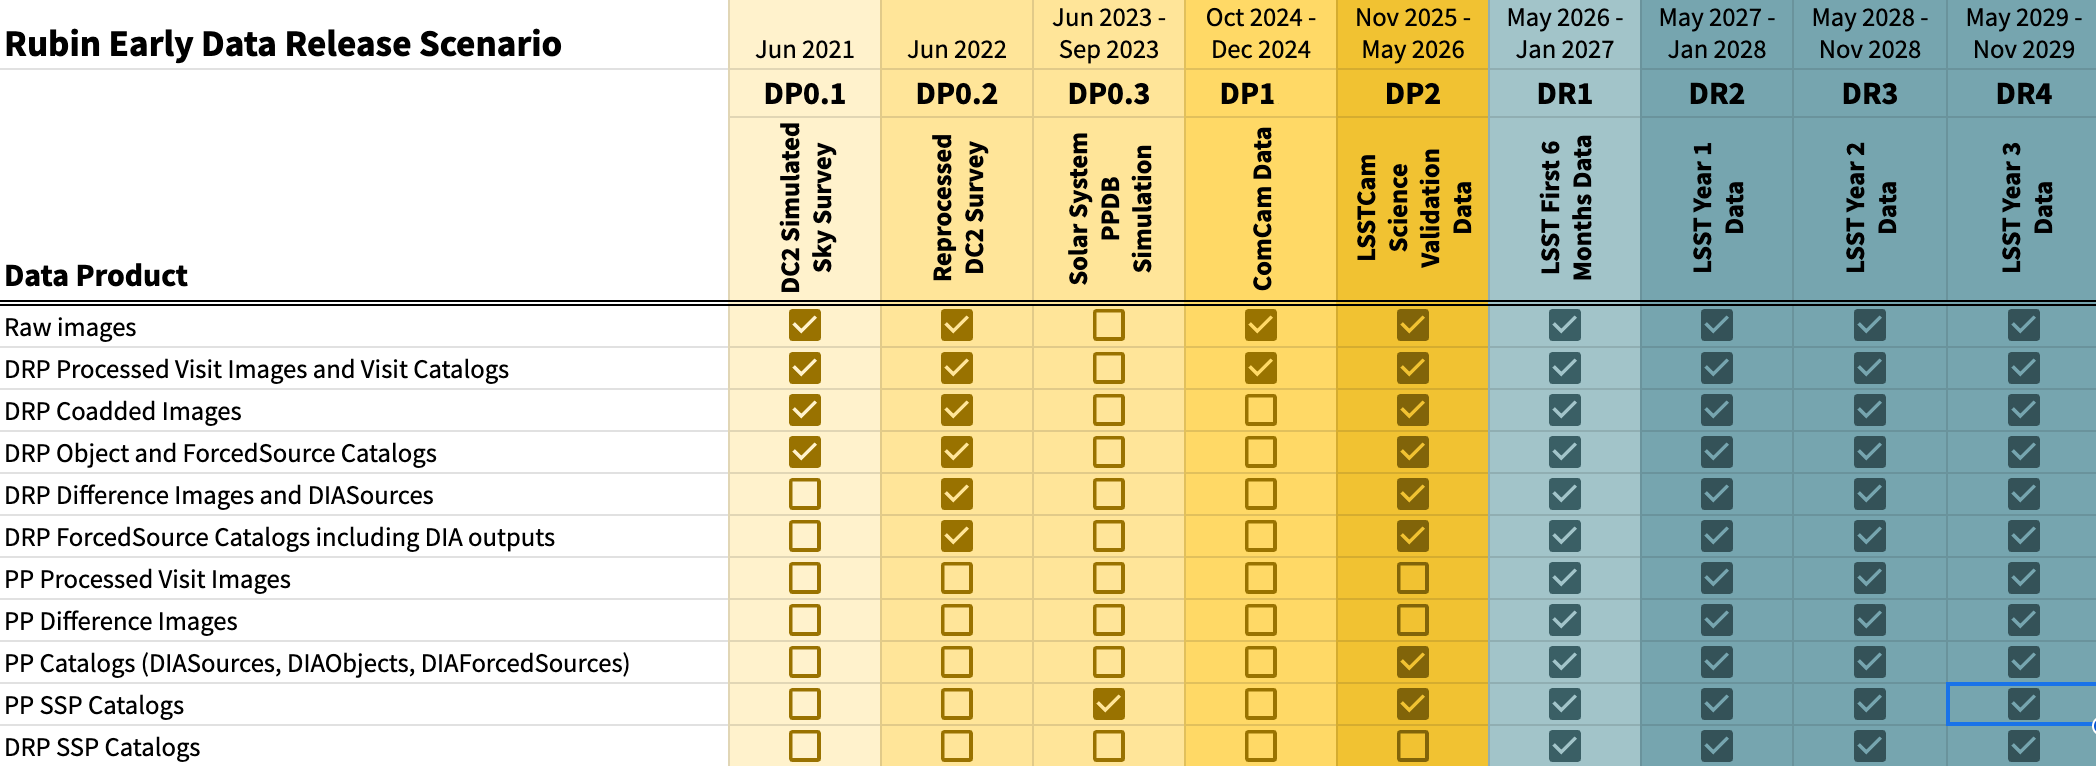
\includegraphics[width=\linewidth]{figures/DPR-summary}
\caption{Summary of data products expected in each data preview and early survey data release, as of January 2023.}
\label{tab:data-preview-summary}
\end{table}

The tables presented in each section below outline which data products can be expected in each Data Preview and Data Release, and on what time scale.
See Table~\ref{tab:milestones} in the Timeline section below for a combined view of the expected data preview schedule and its uncertainties.

\subsection{Data Preview 0}

Data Preview 0 (DP0) is the first of three Data Previews to be released during the period leading up to the start of Rubin Observatory Operations. 
Data Preview 0 contains three stages, all based on simulated LSST-like data products. 
The goals of DP0 are to serve as an early integration test of the LSST Science Pipelines and the Rubin Science Platform (RSP), and to enable a limited number of astronomers and students to begin early preparations for science with the LSST.

\subsubsection{Data Preview 0.1}

Data Preview 0.1 (DP0.1) was released to a group, approximately 300,  of early adopters from the community in June 2021. 
It is based on the the simulated, LSST-like images generated by the Dark Energy Science Collaboration (DESC) for their Data Challenge 2 (DC2), \citep{2021ApJS..253...31L}. 
DP0.1 only uses the 300~\sqdeg of DC2 images that were simulated for five years of the LSST’s wide-fast-deep component (WFD) using a baseline cadence, \citedsp{PSTN-055}.
The DESC processed the simulated DC2 images with \href{https://pipelines.lsst.io/v/v19_0_0/index.html}{Version 19} of the LSST Science Pipelines. 
DP0.1 makes the DESC’s DC2 images and catalogs available to users through an early version the Rubin Science Platform (RSP) running at the US DAC. 

For full details on DP0.1 including an exact description of the data products served, see the documentation at \url{https://dp0-1.lsst.io/}

\subsubsection{Data Preview 0.2}

Data Preview 0.2 (DP0.2) was released to approximately 600 early adopters from the community in June 2022, exactly 1 year after DP0.1. 
The dataset used for DP0.2 was the same as that used for DP0.1.
Rubin processed the simulated DC2 images with \href{https://pipelines.lsst.io/v/v23_0_0/index.html}{Version 23} of the LSST Science Pipelines. 
DP0.2 makes the Rubin reprocessed DESC DC2 images and catalogs available to users through an early version the Rubin Science Platform (RSP) running at the US DAC. 

For full details on DP0.2 including an exact description of the data products served, see the documentation at \url{https://dp0-2.lsst.io/}

\subsubsection{Data Preview 0.3}

Scheduled for between June and September 2023, DP0.3 will be the last in the DP0 series of Data Previews based on simulated LSST-like data. 
The main goal of DP0.3 is to support the Solar System Science Collaboration by hosting their simulated 10-year catalog and serving it via the RSP at the US DAC. 
Table~\ref{tab:dp-zero-three-products} presents a summary of the expected DP0.3 data products, as of January 2023.
The exact data products for DP0.3 are still to be decided. 

\subsection{Data Preview 1}

Data Preview 1 was originally defined to be based on reprocessed on-sky data taken with ComCam.
Following the replan of the Construction project in December 2022, no on-sky data will be taken with ComCam, \S~\ref{sec:commissioning}.
Consequently DP1 has been redefined to be based on a subset of science-grade images taken with LSSTCam during a period of a few days around the System First Light milestone, \S~\ref{ssec:commissioning-observations}.
The processing pipelines and exact data products that will comprise DP1 are still under discussion. 
At minimum, DP1 will deliver visit-level images and catalogs to enable initial studies of observational and instrumental effects. 

Note that the DP1 period of time during which data for DP1 are collected is \textit{very short}: the data products released in DP1 will be generated from relatively few observations taken in the few days around System First Light.
Table~\ref{tab:dp-one-products} presents a summary of the data products expected in DP1, as of January 2023.


\subsection{Data Preview 2}

Data Preview 2 will serve a full consistent reprocessing of all data collected as part of the LSSTCam Science Validation Surveys (SV Surveys) together with any other science-grade commissioning data taken throughout the Science Optimization phase of commissioning, including the DP1 data. 
Table~\ref{tab:dp-two-products} presents a summary of the data products expected in DP1, as of January 2023.

\subsection{Data Release 1}

LSST Data Release 1 will be based on the first six months of data taken as part of the 10-year survey. 
Data Release Processing of this dataset is estimated to to take six months, making the expected delivery date 1 year following the start of the 10 year survey. 
DR1 will be the first Data Release in which all data products will be provided. 

During routine LSST operations, prompt image data products will be made available 80 hours following camera readout.
They include raw images, processed single visit images (PVIs), difference images, and template images.
Access to unvetted PVIs and difference images in the first 6 months of the LSST is still to be decided.

Table~\ref{tab:dr-one-products} presents a summary of the data products expected in DR1, as of January 2023.

\begin{table}[ht]
\centering
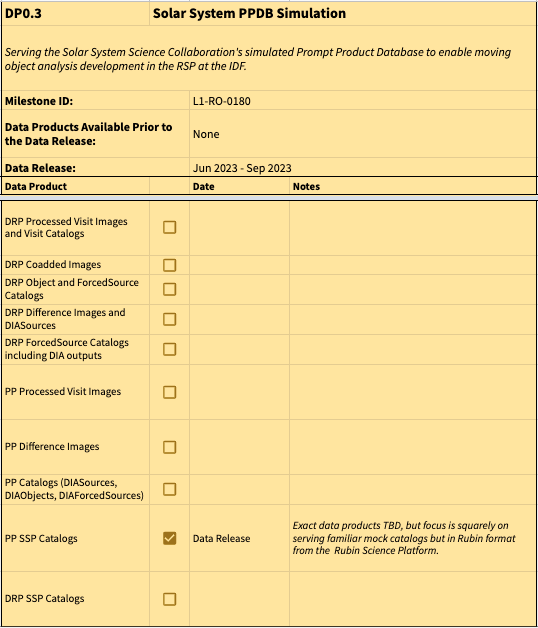
\includegraphics[width=0.9\linewidth]{figures/DP0_3-products.png}
\caption{Summary of data products expected in DP0.3, as of January 2023.}
\label{tab:dp-zero-three-products}
\end{table}

\begin{table}[ht]
\centering
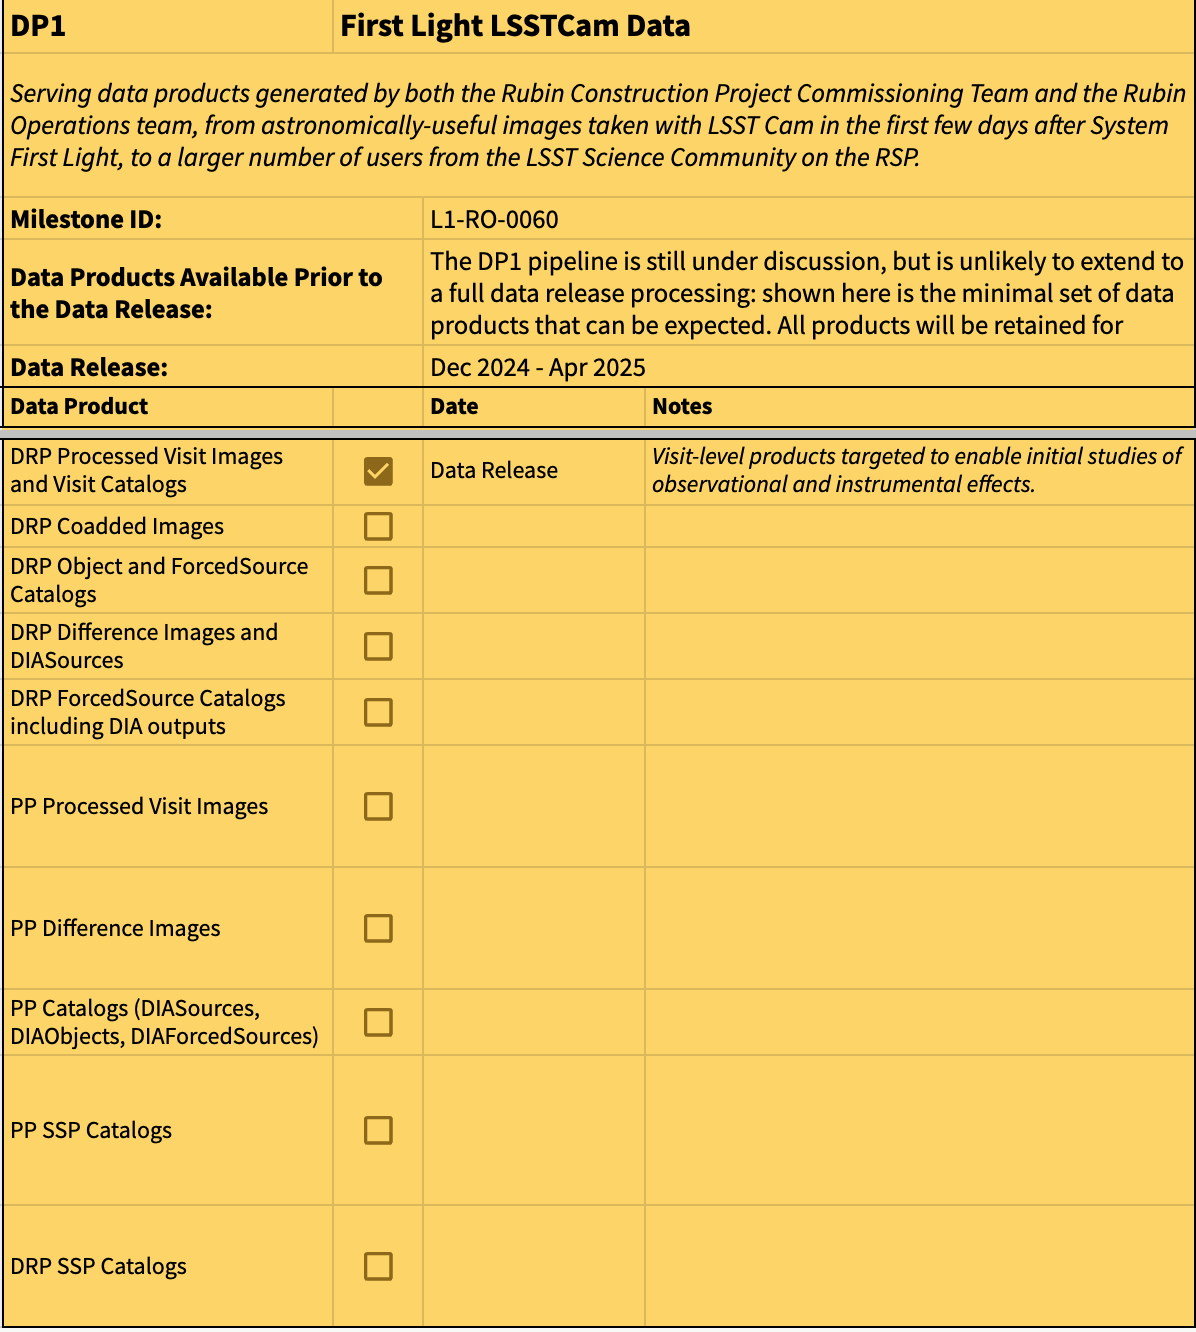
\includegraphics[width=0.9\linewidth]{figures/DP1-products}
\caption{Summary of data products expected in DP1, as of January 2023.
Note the high degree of uncertainty in this table. DP1 will be planned in detail during 2023.}
\label{tab:dp-one-products}
\end{table}

\begin{table}[ht]
\centering
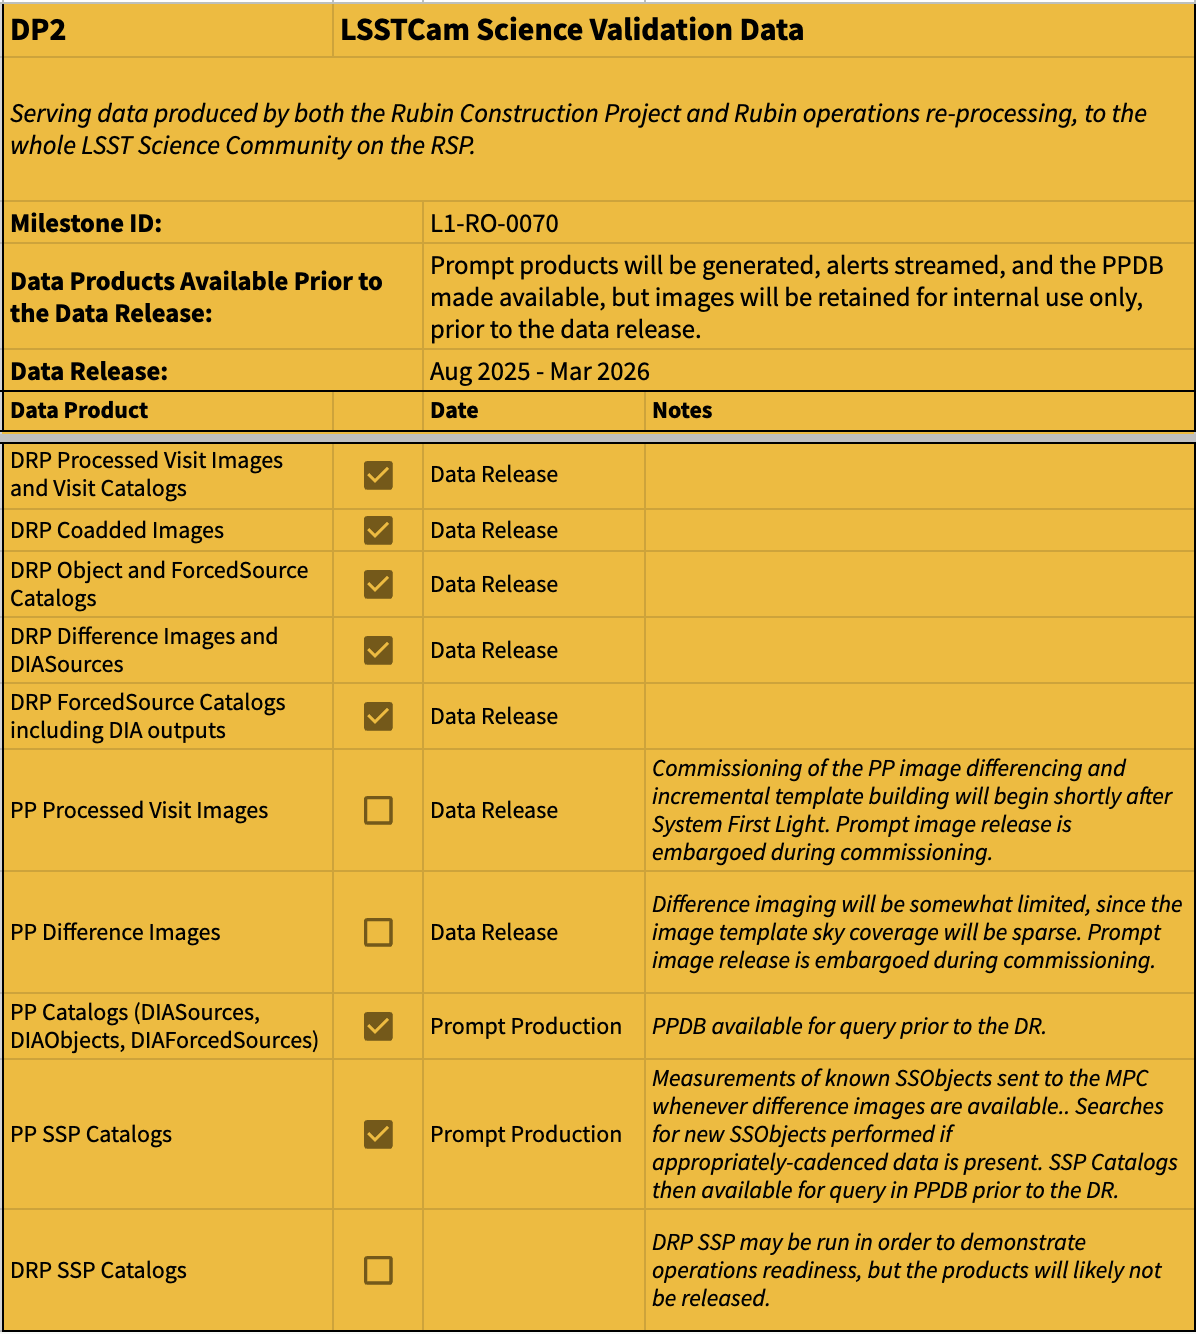
\includegraphics[width=0.9\linewidth]{figures/DP2-products}
\caption{Summary of data products expected in DP2, as of January 2023.}
\label{tab:dp-two-products}
\end{table}

\begin{table}[ht]
\centering
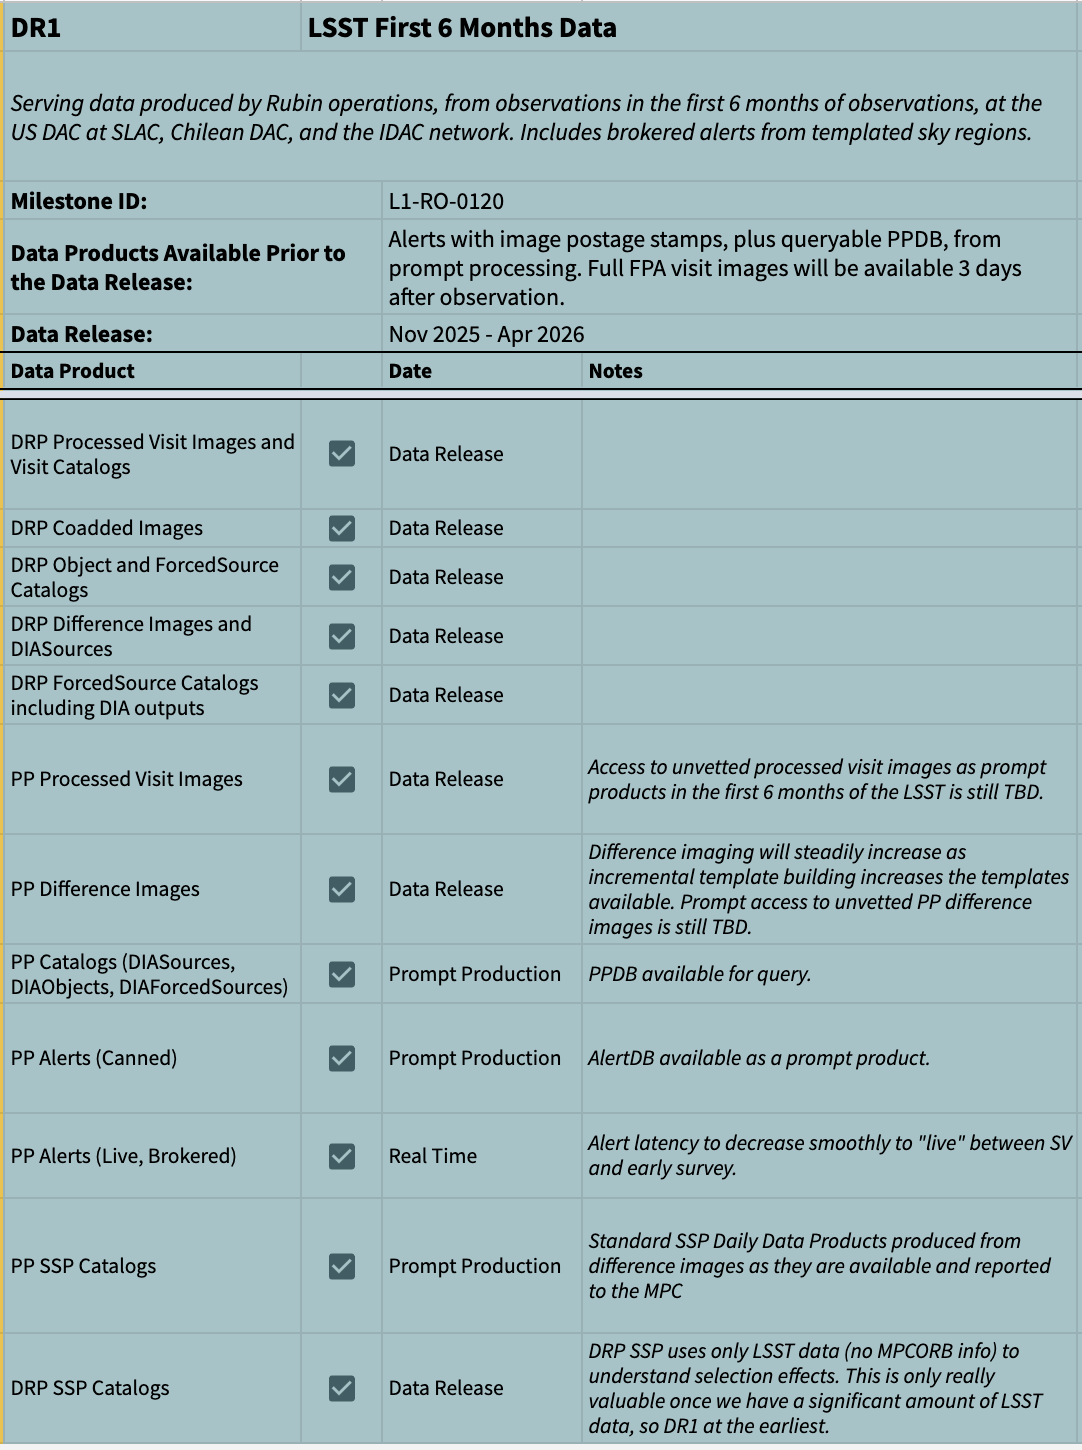
\includegraphics[width=0.9\linewidth]{figures/DR1-products}
\caption{Summary of data products expected in DR1, as of January 2023.}
\label{tab:dr-one-products}
\end{table}

\clearpage
